\entete{HTT}{24 Juin 2011}

\section{Alg\`ebre relationnelle et SQL (10 points)}

Soit le sch\'ema compos\'e des relations suivantes :\\

\smallskip

\texttt{\textbf{ENFANT}(\underline{Num\_enfant}, Nom, Prenom, Annee,
Ville)}\\ 
o\`u \texttt{Num\_enfant} est un num\'ero identifiant un enfant, 
\texttt{Nom} est le nom de famille de l'enfant, \texttt{Prenom} est le
pr\'enom de l'enfant, \texttt{Annee} est l'ann\'ee de naissance de l'enfant, et
\texttt{Ville} est la ville dans laquelle l'enfant vit actuellement.\\

\smallskip

\texttt{\textbf{CRECHE}(\underline{Nom\_creche}, Ville, Capacite)}\\ 
o\`u \texttt{Nom\_creche} est le nom de la cr\`eche,
 \texttt{Ville} est la ville dans laquelle se situe la cr\`eche et 
 \texttt{Capacite} est le nombre maximal d'enfants pouvant
 \^etre accueillis simultan\'ement dans la cr\`eche.\\


\smallskip

\texttt{\textbf{DEMANDE}(\underline{Num\_enfant, Nom\_creche, Annee})}\\ 
est une relation stockant les demandes de place en cr\`eche (pour chaque
ann\'ee). Pour un m\^eme enfant une m\^eme ann\'ee, plusieurs demandes (pour
des cr\`eches diff\'erentes) peuvent \^etre effectu\'ee.\\

\smallskip

\texttt{\textbf{ACCUEIL}(\underline{Num\_enfant, Nom\_creche, Annee}, tarif)}\\ 
est une relation stockant les accueils effectu\'es par les cr\`eches (pour
chaque ann\'ee), en associant le \texttt{tarif} d'accueil (qui peut varier d'une
ann\'ee sur l'autre pour un m\^eme enfant accueilli dans une m\^eme cr\`eche).
On suppose pour simplifier que les enfants sont accueillis par ann\'ee
calendaire. 
%Un enfant ne peut pas \^etre accueilli dans deux cr\`eches diff\'erentes la
%m\^eme ann\'ee. En revanche, un enfant peut \^etre accueilli dans une cr\`eche
%en 2010 et dans une autre cr\`eche en 2011.\\

Pour chaque relation, les attributs soulign\'es forment la clef primaire
de la relation.\\

%NB : si vous estimez que le sujet ne comporte pas l'ensemble des r\`egles de
%gestion permettant la r\'edaction des requ\^etes, vous pouvez poser des
%hypoth\`eses compl\'ementaires. Dans ce cas, indiquez explicitement ces
%hypoth\`eses sur votre copie.\\

%Pour chacune des questions  \'enonc\'ees ci-dessous, vous donnerez une
%expression alg\'ebrique et/ou une requ\^ete SQL (en fonction de ce qui est
%demand\'e) permettant d'y r\'epondre :

\begin{correction} 
Nous donnons ci-dessous quelques corrections possibles. Il peut
exister d'autres corrections bien \'evidemment.
\end{correction}

\begin{enumerate}
  
  \item Quels sont les enfants ayant
   demand\'e en 2010 une place dans (au moins) une cr\`eche de la ville de
   Palaiseau ? Pour r\'epondre \`a cette question, indiquez le num\'ero de
   l'enfant et les noms des cr\`eches de Palaiseau demand\'ees.
  
  \begin{enumerate}
    \item Donnez une expression alg\'ebrique permettant de r\'epondre \`a cette
    question.
\begin{correction} (0,5 pt)\\
      $\Pi_{Num\_enfant, Nom\_creche}(\sigma_{ville='Palaiseau' \wedge
      Annee=2010}(CRECHE \Join DEMANDE))$. On note cette requ\^ete $R_1$ dans la suite.
\end{correction}
    \item Donnez une requ\^ete SQL permettant de r\'epondre \`a cette
    question.
 \begin{correction} (0,5 pt)
      \begin{lstlisting}[language=SQL]
Select Num_enfant, CRECHE.Nom_creche
From CRECHE, DEMANDE
Where CRECHE.Nom_creche=DEMANDE.Nom_creche and Ville='Palaiseau' and Annee=2010
      \end{lstlisting}
      
      ou
            \begin{lstlisting}[language=SQL]
Select Num_enfant, Nom_creche
From CRECHE NATURAL JOIN DEMANDE
Where Ville='Palaiseau' and Annee=2010
      \end{lstlisting}
\end{correction}
  \end{enumerate}
  
  
  \item Quels sont les nom et pr\'emon des enfants n\'es en 2009 ayant
  d\'ej\`a \'et\'e accueillis dans une cr\`eche (en n'importe quelle ann\'ee) ?
  
  \begin{enumerate}
      \item Donnez une expression alg\'ebrique permettant de r\'epondre \`a cette
    question.
\begin{correction} (1 pt)\\
	Soit la requ\^ete $R$ suivante, jointure des relations $ENFANT$ et $ACCUEIL$:\\
      $R : ENFANT
      \Join_{ENFANT.Num\_enfant=ACCUEIL.Num\_enfant} ACCUEIL$\\
      Attention ici dans $R$, la
      jointure ne doit pas \^etre naturelle \`a cause de l'attribut \texttt{Annee} sur lequel on ne veut pas joindre !\\
      Une correction est $\pi_{Nom,Prenom}(\sigma_{ENFANT.Annee=2009}(R))$.\\
      ou \\ (avec renommage explicite pour pouvoir effectuer
      une jointure naturelle) : \\$\sigma_{Annee\_naiss=2009}(\rho_{Annee
      \rightarrow Annee\_naiss}(ENFANT) \Join ACCUEIL)$\\
  ou encore \\
      $\pi_{Nom,Prenom}(\pi_{Num\_enfant,
      Nom, Prenom}(\sigma_{Annee=2009}(ENFANT))) \Join ACCUEIL)$.
\end{correction} 
    \item Donnez une requ\^ete SQL permettant de
    r\'epondre \`a cette question.
\begin{correction} (1 pt)
      \begin{lstlisting}[language=SQL]
Select ENFANT.Nom, ACCUEIL.Prenom
From ENFANT, ACCUEIL
Where ENFANT.Num_enfant=ACCUEIL.Num_enfant and ENFANT.Annee=2009
      \end{lstlisting}
\end{correction}
  \end{enumerate}
 
   \item Quels sont les num\'eros des enfants ayant demand\'e toutes les
   cr\`eches de la ville de Palaiseau en 2010 ?
  \begin{enumerate}
      \item Donnez une expression alg\'ebrique permettant de
      r\'epondre \`a cette question.
\begin{correction} (1,5 pt)\\
	Soit $R_2$ la requ\^ete suivante recup\'erant les noms de toutes les cr\`eches
	de Palaiseau : \\
	$R_2 : \Pi_{Nom\_creche}(\sigma_{Ville='Palaiseau'}(CRECHE))$.\\
	On utilise ensuite la requ\^ete $R_1$ d\'efinie pr\'ec\'edemment :
	$\Pi_{Num\_enfant}(R_1 \div R_2)$ \\
%	ou bien \\
%	$\Pi_{Num\_enfant, Nom\_creche}(\sigma_{
 %     Annee=2010}(DEMANDE)) \div \Pi_{Num\_enfant}(R_1 \div R_2)$ 
\end{correction}

  
 (Attention, vous ne donnez pas de requ\^ete SQL correspondante pour cette
question).
 
  \end{enumerate}

   \item Combien d'enfants ont \'et\'e accueillis en 2010 par les cr\`eches de
   la ville de Paris ?
  \begin{enumerate}
      \item Donnez une requ\^ete SQL permettant de r\'epondre \`a cette
    question.
\begin{correction} (1 pt)
     \begin{lstlisting}[language=SQL]
     Select count(*) 
     From CRECHE, ACCUEIL
     Where Ville='Paris' and CRECHE.Nom_creche=ACCUEIL.Nom_creche and Annee=2010
     \end{lstlisting}
\end{correction}
  \end{enumerate}
   (Attention, vous ne donnez pas d'expression alg\'ebrique correspondante pour
   cette question).
  
    
  \item Quels sont les noms et pr\'enoms des enfants pour lesquels il n'a jamais
  \'et\'e d\'epos\'e de demande de cr\`eche (pour aucune ann\'ee) ?
  
  \begin{enumerate}
      \item Donnez une expression alg\'ebrique permettant de r\'epondre \`a cette
    question.
\begin{correction} (1 pt)\\
      $\Pi_{Nom,Prenom}((\underbrace{\underbrace{\Pi_{Num\_enfant}(ENFANT)}_{\text{Tous
      les
      enfants}}-\underbrace{\Pi_{Num\_enfant}(DEMANDE)}_{\text{Enfants
      apparaissant dans une demande}}}_{\text{Num\_enfant des enfants pour
      lesquels il n'existe pas de demande}}) \underbrace{\Join
      ENFANT}_{\text{Recup. Nom et Prenom}})$\\
\end{correction}
    \item Donnez une requ\^ete SQL avec imbrication permettant de
    r\'epondre \`a cette question.
\begin{correction} (1,5 pt)
      \begin{lstlisting}[language=SQL]
	Select Nom, Prenom
	From ENFANT
	Where Num_enfant Not In (Select Num_enfant from DEMANDE)
      \end{lstlisting}
\end{correction}
  \end{enumerate}
  
  \item Quelles sont les cr\`eches n'ayant pas rempli toutes leurs places
  (c.f. la \texttt{Capacite} d'une cr\`eche) en 2010 ?
  
  \begin{enumerate}
    \item Donnez une requ\^ete SQL permettant de
    r\'epondre \`a cette question.
\begin{correction} (2 pts)
      \begin{lstlisting}[language=SQL,emph={CRECHE}, emphstyle=\textit]
	Select Nom_creche
	From CRECHE
	Where Capacite > (Select count(*) 
				From ACCUEIL 
				Where Annee=2010 and Nom_creche=CRECHE.Nom_creche)
      \end{lstlisting}
\end{correction}
  \end{enumerate}
  
  
    \end{enumerate}
 
% \end{enumerate}
 
\section{Index et optimisation  (5 points)}

\begin{enumerate}
  \item On souhaite cr\'eer un index B+Tree d'ordre 2 sur les
  capacit\'es des cr\`eches. Donner les diff\'erentes \'etapes d'\'eclatement de l'arbre apr\`es l'insertion successive des valeurs suivantes:
  \begin{center}
  200, 150, 250, 300, 220, 350, 240, 300, 400, 50, 100
  \end{center}
\begin{correction}
  \begin{figure}[htbp]
  \centering
  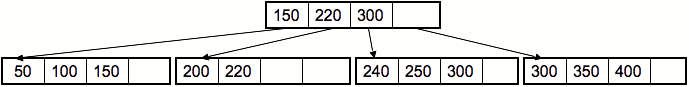
\epsfig{file=Fig/2010-2011_btree.eps, width=12cm}
  \end{figure}
\end{correction}
 
  \item Soit la requ\^ete suivante:
      \begin{lstlisting}[language=SQL]
     Select Nom, Prenom 
     From ENFANT, ACCUEIL
     Where ENFANT.Num_enfant = ACCUEIL.Num_enfant AND
           ENFANT.annee = 2009 AND
           ACCUEIL.annee = 2019 AND
           ENFANT.VILLE = 'Paris'
     \end{lstlisting}
     Donner un plan d'ex\'ecution (arborescente ou EXPLAIN) produit par l'optimiseur 
     en argumentant votre r\'eponse, sachant qu'il existe:
     \begin{itemize}
       \item Un index sur l'ann\'ee d'ACCUEIL;
       \item La table ENFANT compte 1000 pages 
       \item La table ACCUEIL compte 100 pages
     \end{itemize}
     Vous ajouterez les pr\'edicats associ\'es \`a chaque op\'erateur en dessous du
     plan.
\begin{correction}
     Comme il y a une grosse diff\'erence entre Enfant et Accueil, nous utiliserons un NESTED LOOP JOIN, et l'index sur accueil sera utilis\'e.
    \begin{verbatim}
    0 SELECT STATEMENT
    1*  NESTED LOOP JOIN
    2     TABLE ACCESS BY INDEX ROWID  ACCUEIL
    3*      INDEX RANGE SCAN           IDX_ACCUEIL_ANNEE
    4*    TABLE ACCESS FULL            ENFANT
 
    (1) ENFANT.Num_enfant = ACCUEIL.Num_enfant
    (3) ACCUEIL.annee = 2010
    (4) ENFANT.annee = 2009 AND ENFANT.VILLE = 'Paris'
    \end{verbatim}
\end{correction}

	\item Nous ajoutons maintenant un index sur ENFANT.Num\_enfant. Proposer un plan d'ex\'ecution (arborescente ou EXPLAIN) en prenant en compte cet index.
\begin{correction}
    ~
    \begin{verbatim}
    0 SELECT STATEMENT
    1   NESTED LOOP JOIN
    2     TABLE ACCESS BY INDEX ROWID  ACCUEIL
    3*      INDEX RANGE SCAN           IDX_ACCUEIL_ANNEE
    4*    TABLE ACCESS BY INDEX ROWID  ENFANT
    5*      INDEX RANGE SCAN           IDX_ENFANT_NUM_ENFANT

    (3) ACCUEIL.annee = 2010
    (4) ENFANT.annee = 2009 AND ENFANT.VILLE = 'Paris'
    (5) ENFANT.Num_enfant = ACCUEIL.Num_enfant
    \end{verbatim}
\end{correction}
\end{enumerate}	

\section{Concurrence (5 points)}


L'ex\'ecution suivante est re\c{c}ue par un SGBD\,:

$$H : r_1[x] r_2[z] r_1[y] w_1[x] r_3[x] r_2[y] w_2[z] w_2[y] c_2 r_3[y] r_3[z] c_3 w_1[y] c_1 $$

\begin{enumerate}
  \item  Parmi les transactions $T_1$, $T_2$, $T_3$, certaines correspondent
     au virement d'un compte vers un autre\,: on lit les 
    valeurs des deux comptes, puis on les modifie. De quelles
         transactions s'agit-il\,?

\begin{correction}
      $T_1$ et $T_2$.
\end{correction}

  \item  Existe-t-il des ``lectures sales'' (lecture par une transaction
  d'une donn\'ee modifi\'ee par une autre, mais pas encore valid\'ee) dans $H$\,?
  Indiquez-les, ainsi que les cons\'equences possibles.
\begin{correction}
r3[x] apr\`es w1[x]. Si T1 s'annule \`a la place de valid\'ee, la donn\'ee lue en w3[x] est incoh\'erente.
\end{correction}

  \item  V\'erifiez si $H$ est s\'erialisable en 
    identifiant les conflits et en construisant le graphe de s\'erialisation.
\begin{correction}
      Les conflits :
      sur x : w1[x]-r3[x]
      sur y : r1[y]-w2[y], w2[y] r3[y] w2[y]-w1[y]
      sur z : w2[z] r3[z]

      Le graphe de s\'erialisation contient un cycle T1 T2, 
      donc H n'est pas s\'erialisable.
\end{correction}

\item  Qu'obtient-on en appliquant un verrouillage \`a 
       deux phases \`a partir de $H$ (indiquer le d\'eroulement de l'ex\'ecution,
        et les blocages \'eventuels)\,?

\begin{correction}
   On arrive \`a interblocage\,: verrouillage en lecture de $T_2$ sur $y$, quand
    $T_1$ cherche \`a \'ecrire.
\end{correction}

\item On suppose maintenant que toutes les transactions
    placent un \texttt{FOR UPDATE} pour toute lecture
    d'une donn\'ee {\em qui va \`a \^etre modifi\'ee ensuite}.  Qu'obient-on 
     si on applique \`a $H$ 
    une variante du verrouillage \`a deux phases
    qui pose un verrou exclusif (au lieu d'un verrou partag\'e) pour les
    lectures comprenant la clause \texttt{FOR UPDATE}\,? 

\begin{correction}
   $T_1$ pose des verrous exclusifs qui mettent les autres transactions
en attente.
 Ensuite tout se passe bien.
\end{correction}

\end{enumerate}